\subsubsection{Map Operations}
\label{ref:osgview_map_ops}

To access the map operations, click the globe symbol 
\includegraphics[width=0.5cm,frame]{../../data/icons/globe.png}. Please note that only the main Map item has a context menu, and only allows setting of map files and changing of the opacity.

\begin{itemize}
 \item Map File: Change the background map
 \item Opacity: Change the background map opacity
\end{itemize} 

\paragraph{Changing the Background Map}

Please note that, while the default background map is supplied ATSDB, the other background map types are downloaded from public Internet sources and therefore require an Internet connection. They are then cached locally to facilitate faster access. \\

For each map layer defined in the background map, a checkbox is shown to disable the layer, and by clicking on the map layer symbol it's opacity can be changed.

To change the background map, click the globe symbol 
\includegraphics[width=0.5cm,frame]{../../data/icons/globe.png} in root Map layer to access the map selection. \\

The following maps are commonly available:

\begin{itemize}
 \item arcgis.earth*
 \item minimal.earth*
 \item openstreetmap.earth*
 \item openstreetmap\_german.earth*
 \item readymap.earth
 \item readymap-detailed.earth
\end{itemize}
 \ \\
 
 Please note that for each map marked with \textbf{*} a 3D version (as listed) and a 2D version (with filename suffix '\_2d') exists. Each of them contains similiar content, but changes the display mode to 3D/2D upon selection. \\
 
The map loading and display in based on the osgEarth library (\url{http://osgearth.org/}), as are to map file definitions.  \\

The map which can be set using this dialog is simply a file list from the folder '\textasciitilde/.atsdb/data/maps'. So, changes can be made to the supplied ones or custom user maps can be added to this folder. \\
Please refer to section \nameref{sec:adding_maps} for further details.

\newpage
\paragraph{ArcGIS Map}

As supplied in the osgEarth example files, this map data is obtained from ArcGIS Online (\url{https://doc.arcgis.com/en/arcgis-online/reference/what-is-agol.htm}). It shows satellite imagery, supplied with elevation data from ReadyMap. 

\begin{figure}[H]
    \hspace*{-2.5cm}
    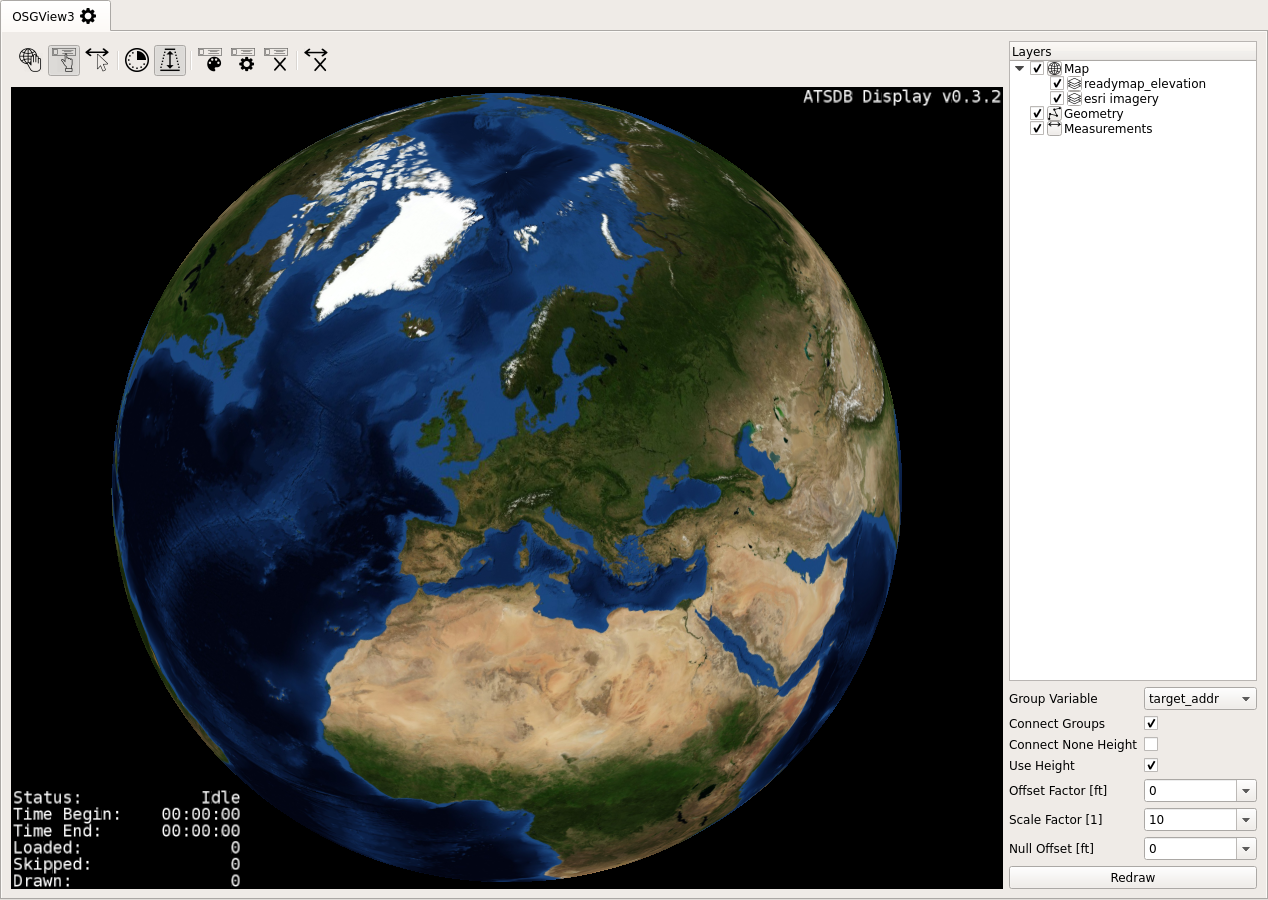
\includegraphics[width=19cm,frame]{../screenshots/osgview_arcgis.png}
  \caption{OSG View Arcgis map}
\end{figure}

\newpage
\paragraph{Minimal Map}

This minimal map shows national borders based on an ESRI shapefile, provided by Bjorn Sandvik on \url{thematicmapping.org} and European airports, provided by \url{https://ec.europa.eu/eurostat/web/gisco/geodata/reference-data/transport-networks}.

\begin{figure}[H]
    \hspace*{-2.5cm}
    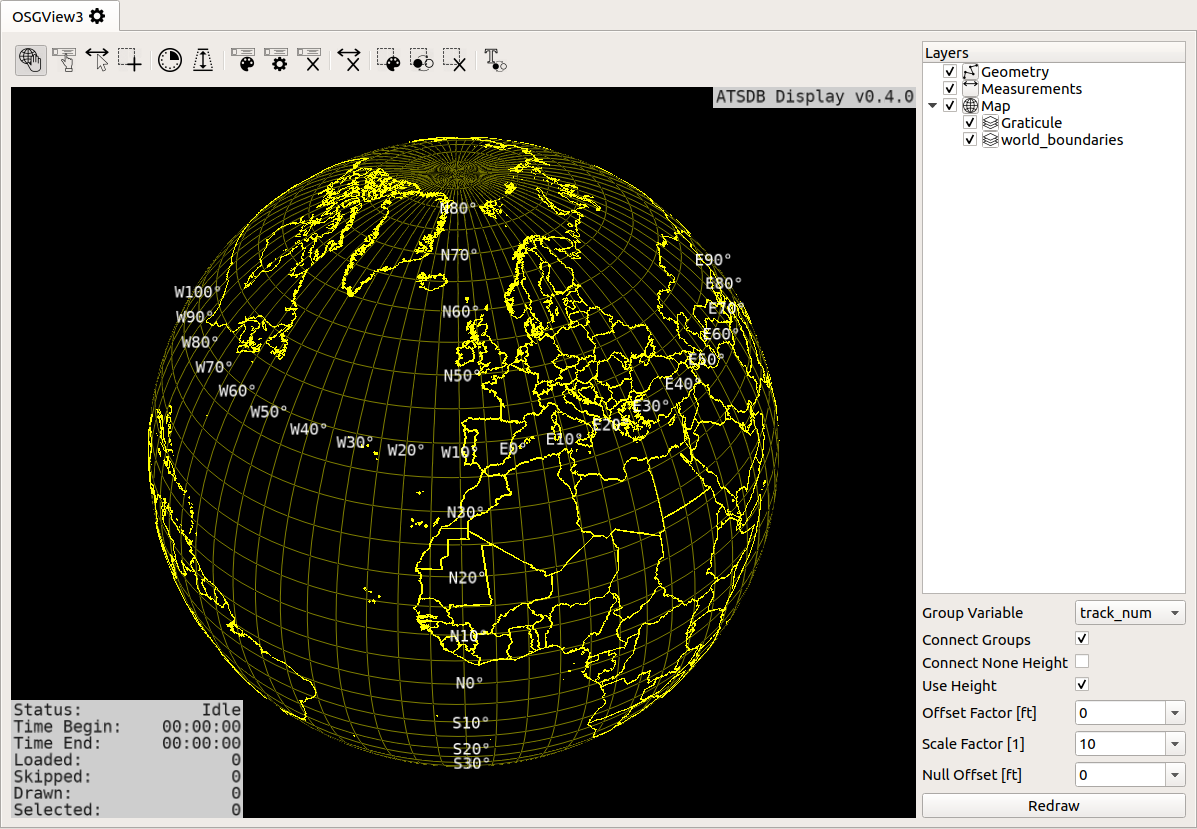
\includegraphics[width=19cm,frame]{../screenshots/osgview_minimal.png}
  \caption{OSG View minimal map}
\end{figure}

\newpage
\paragraph{Open Street Map}

This very useful map shows map data from \url{https://www.openstreetmap.org/}.

\begin{figure}[H]
    \hspace*{-2.5cm}
    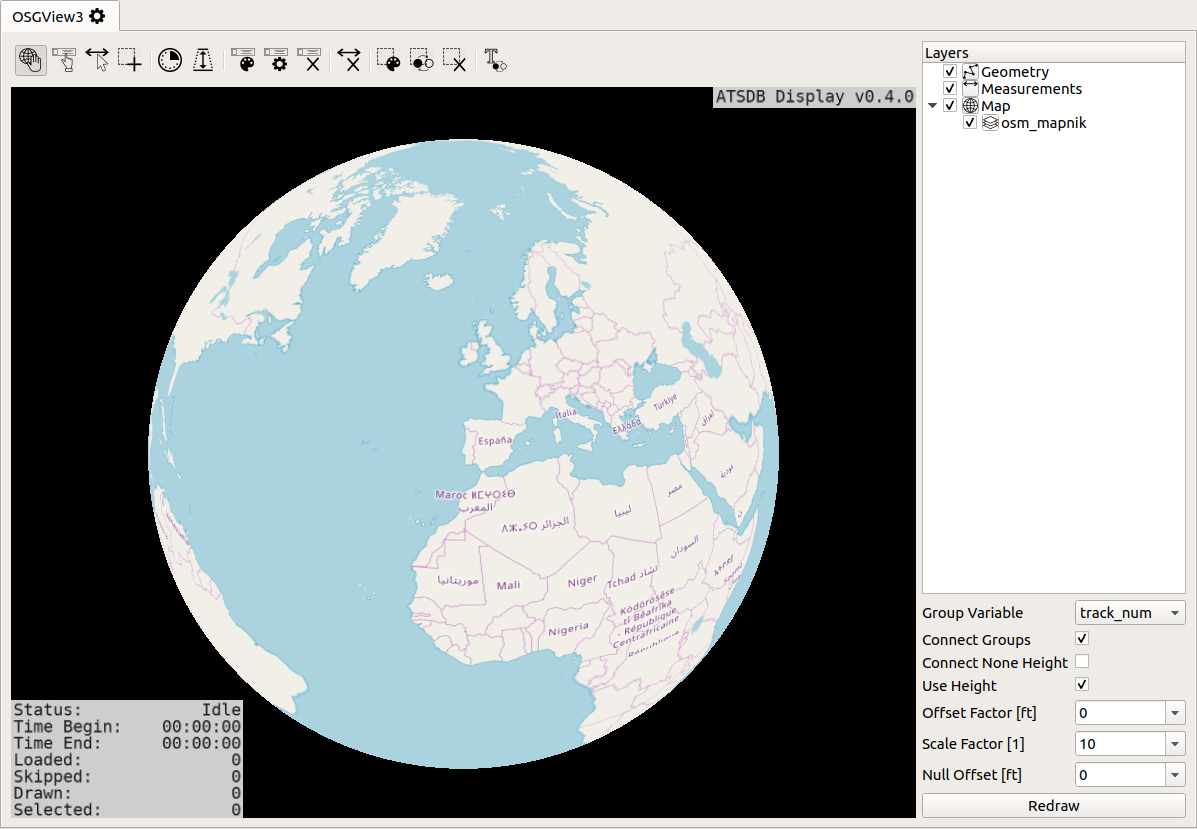
\includegraphics[width=19cm,frame]{../screenshots/osgview_osm.png}
  \caption{OSG View OpenStreetMap}
\end{figure}

It is possible to zoom in to a very high level of detail, to even inspect airport layouts.

\begin{figure}[H]
    \hspace*{-2.5cm}
    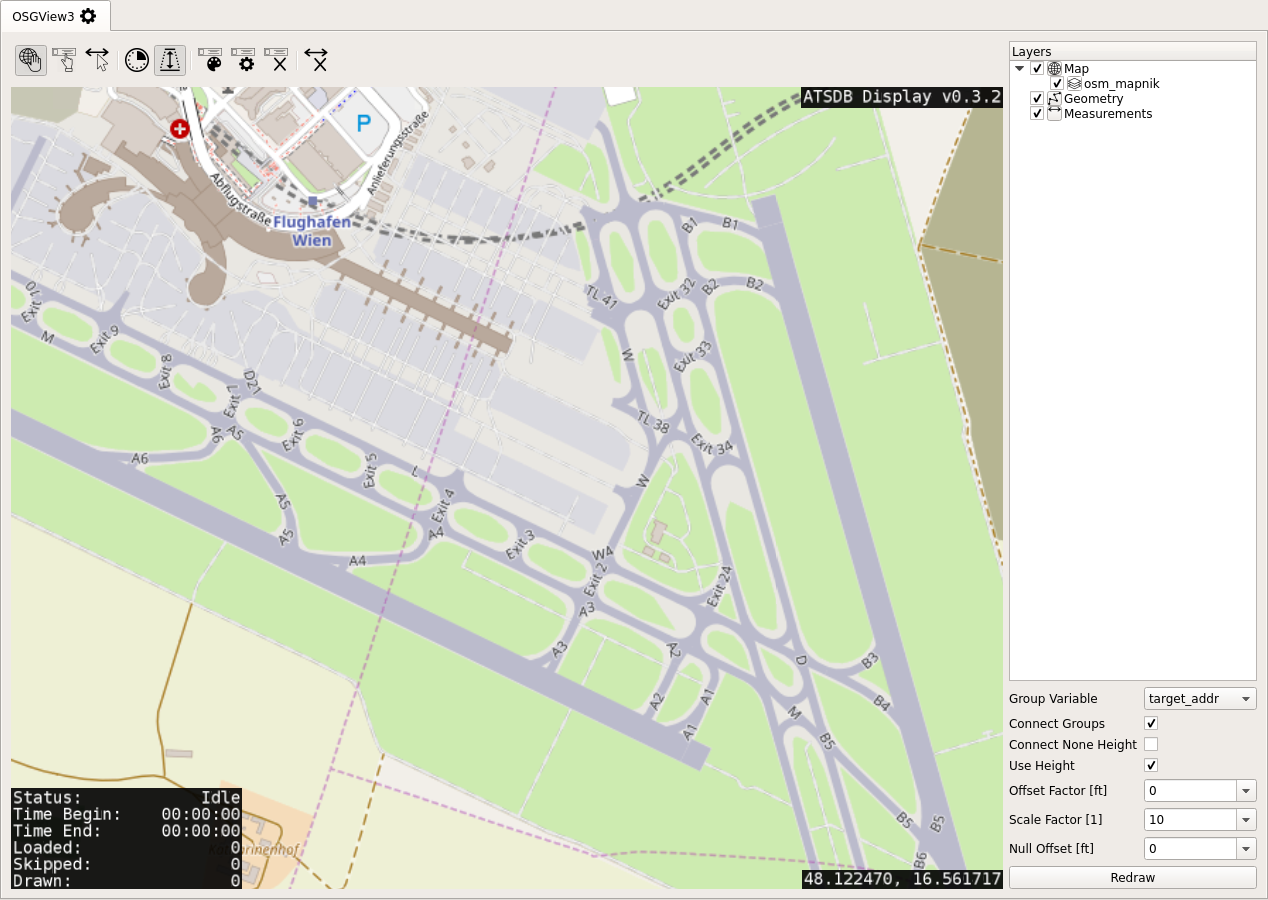
\includegraphics[width=19cm,frame]{../screenshots/osgview_osm_vienna.png}
  \caption{OSG View OpenStreetMap Vienna Airport}
\end{figure}

\newpage
\paragraph{Open Street Map German}

This very useful map shows map data from \url{https://www.openstreetmap.de/}.

\begin{figure}[H]
    \hspace*{-2.5cm}
    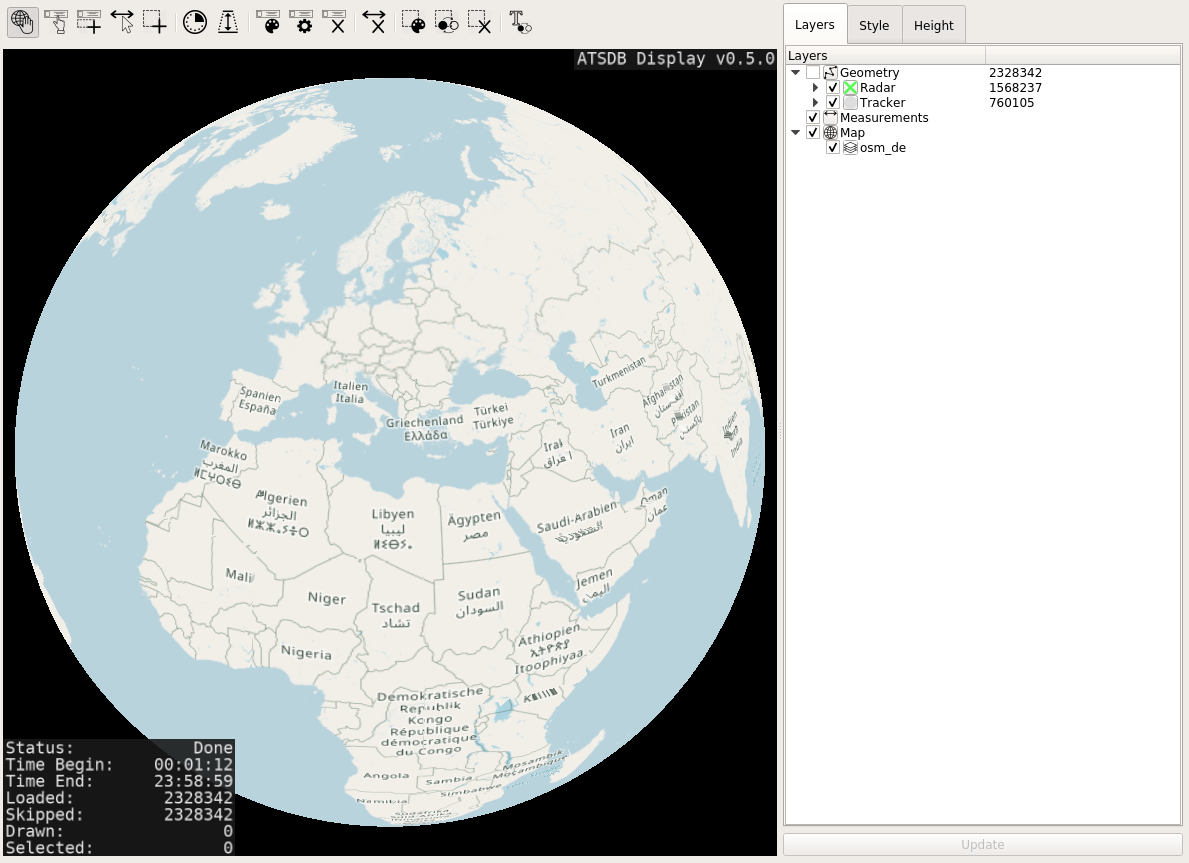
\includegraphics[width=19cm,frame]{../screenshots/osgview_osm_de.png}
  \caption{OSG View OpenStreetMap German}
\end{figure}

It is possible to zoom in to a very high level of detail, to even inspect airport layouts.

\newpage
\paragraph{ReadyMap \& ReadyMap Detailed}

This map also shows satellite data, from \url{http://web.pelicanmapping.com/readymap-tiles/}.

\begin{figure}[H]
    \hspace*{-2.5cm}
    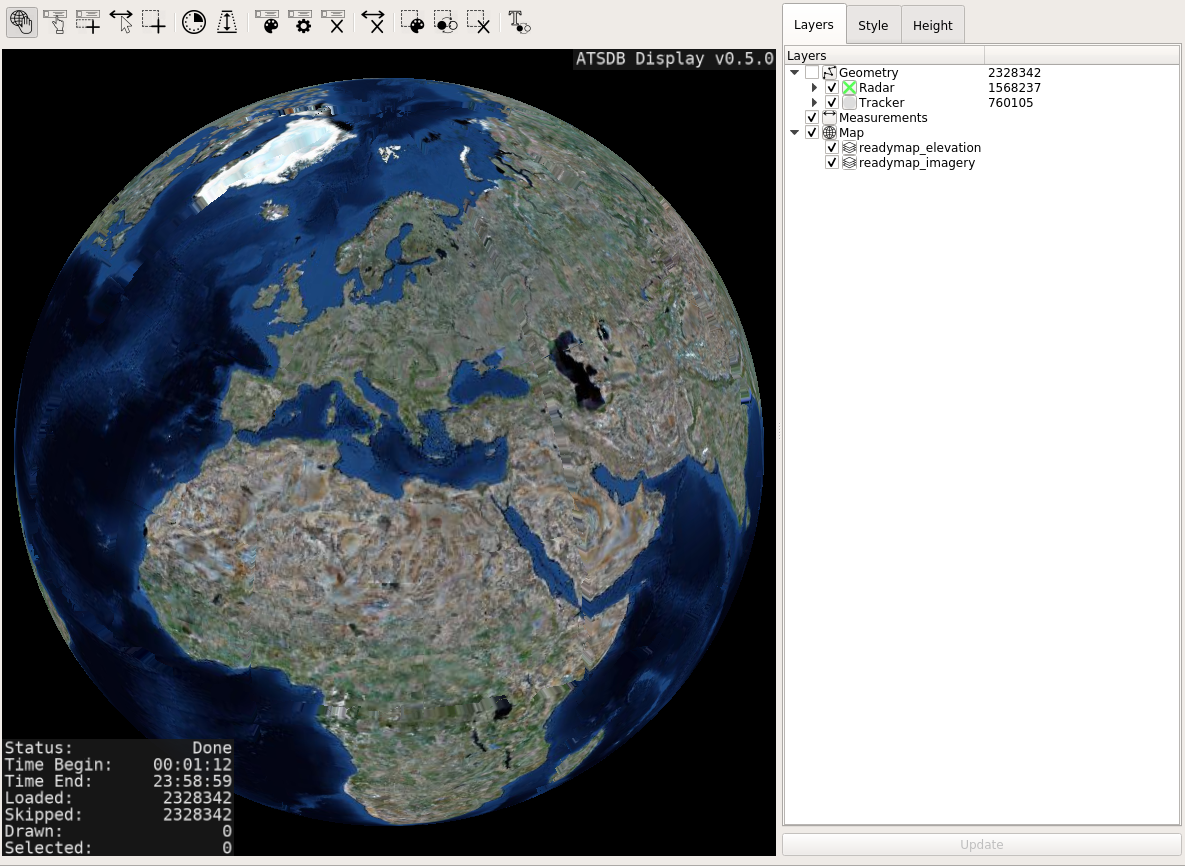
\includegraphics[width=19cm,frame]{../screenshots/osgview_ready.png}
  \caption{OSG View ReadyMap}
\end{figure}

This detailed version shows the same data as ReadyMap, but to a higher detail level. \\

Please note that this map includes an elevation layer, so mountains are modeled in 3D.

\begin{figure}[H]
    \hspace*{-2.5cm}
    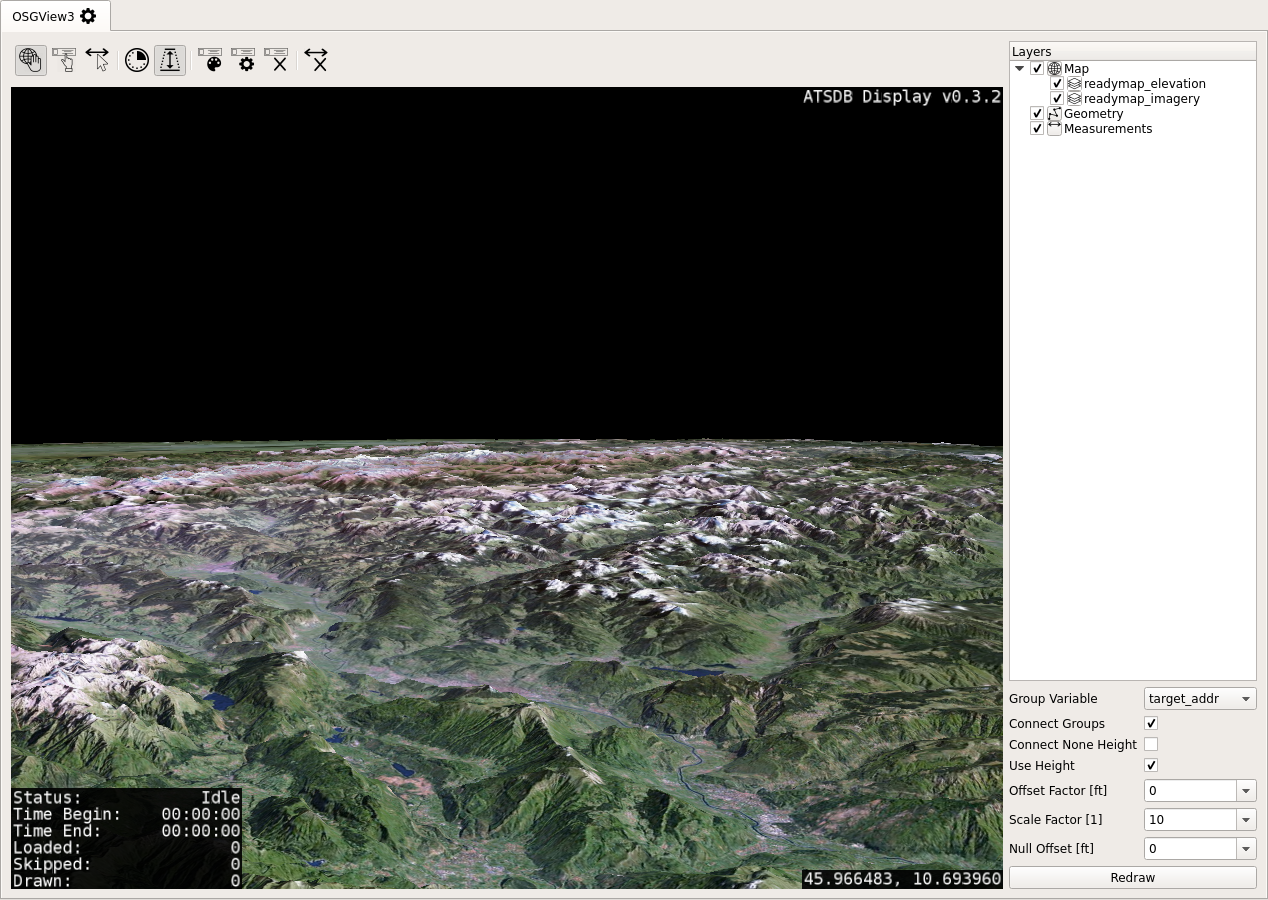
\includegraphics[width=19cm]{../screenshots/osgview_readymap_elav.png}
  \caption{OSG View ReadyMap detailed elevation}
\end{figure}

\paragraph{Adding/Changing Map Files}
\label{sec:adding_maps}

As with all configuration, a local version is kept in the home folder of the user. The map files are loaded from the hidden folder '\textasciitilde/.atsdb/data/maps' ('\textasciitilde' is the user's home directory, like /home/user).

\begin{figure}[H]
    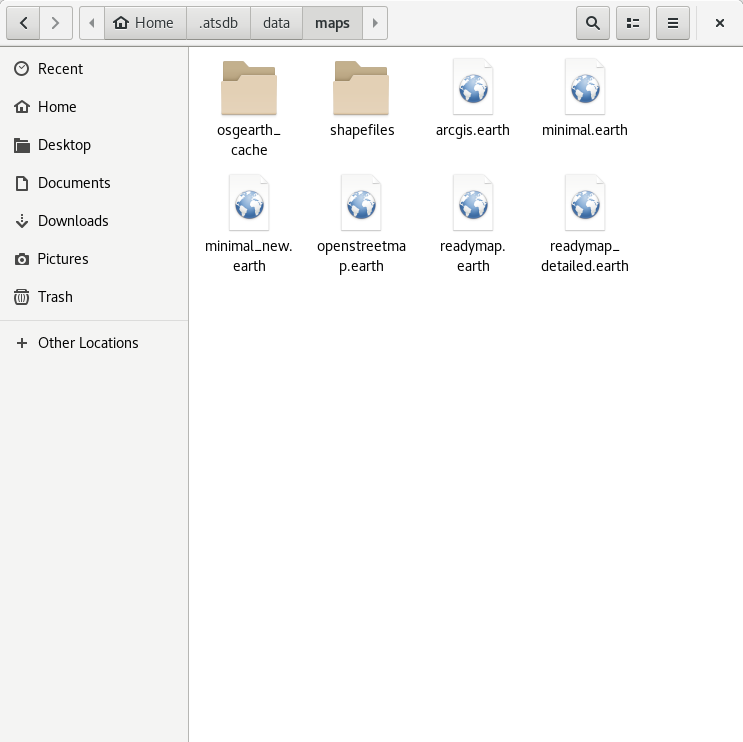
\includegraphics[width=10cm,frame]{../screenshots/maps_config.png}
  \caption{Maps Folder}
\end{figure}

In this folder, the previosly discussed maps exist as osgEarth '.earth' files. If new .earth files are added, or the content of such files is changed, they can be used from the OSGView after a restart.

The easiest example is the 'minimal\_new.earth' file, which uses an ESRI shapefile from the subfolder 'shapefiles' to display the national borders.

\begin{lstlisting}
<map name="Wordwide Line Vectors" type="geocentric">
  
    <options>
        <lighting>false</lighting>
        <terrain>
            <min_tile_range_factor>8</min_tile_range_factor>
            <color>#000000FF</color>
        </terrain>
      
    </options>

    <feature_source name="world-data" driver="ogr">
        <url>shapefiles/TM_WORLD_BORDERS-0.3.shp</url>
        <convert type="line"/>
    </feature_source>
    
    <feature_model name="world_boundaries" feature_source="world-data">
        
        <layout tile_size="100000"  paged="true">
            <level max_range="1e10"/>
        </layout>
                
        <styles>
            <style type="text/css">
                world {
                   stroke:                   #ffff00;
                   stroke-width:             2px;
                   stroke-tessellation-size: 1km;
                   render-lighting:          false;
                   altitude-clamping:        none;
                   render-depth-test: false;
                }            
            </style>
        </styles>
        
    </feature_model>
 

</map>
\end{lstlisting}

The world background colour is set using the 'terrain color' tag. The name of the shapefile is given using the 'url' tag, the line colour and width is set in the style below. Basically a user can add their own files to the 'shapefiles' folder, and simply duplicate the 'feature\_model' part with their own ESRI shapefiles. This could the look like this:

\begin{lstlisting}
<map name="Wordwide Line Vectors" type="geocentric">
  
    <options>
        <lighting>false</lighting>
         <terrain color="#101010ff"/>
    </options>

    <feature_source name="world-data" driver="ogr">
        <url>shapefiles/TM_WORLD_BORDERS-0.3.shp</url>
        <convert type="line"/>
    </feature_source>
    
    <feature_model name="world_boundaries" feature_source="world-data">
        
        <layout tile_size="100000"  paged="true">
            <level max_range="1e10"/>
        </layout>
                
        <styles>
            <style type="text/css">
                world {
                   stroke:                   #ffff00;
                   stroke-width:             2px;
                   stroke-tessellation-size: 1km;
                   render-lighting:          false;
                   altitude-clamping:        none;
                   render-depth-test: false;                   
                }            
            </style>
        </styles>
        
    </feature_model>
  
    <feature_model name="doi">
        <features name="wolrd" driver="ogr">
            <url>shapefiles/doi.shp</url>
            <build_spatial_index>true</build_spatial_index>
            <ogr_driver>ESRI Shapefile</ogr_driver>
            <convert type="line"/>
        </features>        

        <layout tile_size="100000">
            <level max_range="1e10"/>
        </layout>

        <styles>
            <style type="text/css">
                states {
                   stroke:          #00ff00; 
                   stroke-width:    2px;
                   render-depth-test: false;
                }                    
            </style>
        </styles>        
    </feature_model>
</map>
\end{lstlisting}

While a number of formats are supported, to add a KML file, add the following part to a 'map' (as previously):

\begin{lstlisting}
     <feature_model name="wam_area">
        <features name="wam_area" driver="ogr">
            <url>shapefiles/wam_area.kml</url>
            <ogr_driver>LIBKML</ogr_driver>
            <build_spatial_index>true</build_spatial_index>
        </features>        

        <styles>
            <style type="text/css">
                states {
                   stroke:          #0000ff; 
                   stroke-width:    2px;
                   render-depth-test: false;
                }                    
            </style>
        </styles>        
    </feature_model>
\end{lstlisting}

To add a GML file, add the following part to a 'map' (as previously):

\begin{lstlisting}
   <model driver="feature_geom" name="gml" cache_enabled="false">
    <features driver="ogr">
	<ogr_driver>GML</ogr_driver>
        <url>shapefiles/example.gml</url>
        <caching_policy usage="no_cache"/>
    </features>
   </model>
\end{lstlisting}

To add a GeoTIFF file, add the following part to a 'map' (as previously):

\begin{lstlisting}
    <image driver="gdal" name="tiff" cache_enabled="false" visible="false">
        <url>/usr/share/osgearth/data/world.tif</url>
        <caching_policy usage="no_cache"/>
    </image>
\end{lstlisting}

To add a graticule (latitude/longitude grid), add the following part to a 'map' (as previously):

\begin{lstlisting}
    <geodetic_graticule name="Graticule" visible="true">
        <color>#ffff007f</color>
        <label_color>#ffffffff</label_color>
        <grid_lines>20</grid_lines>
        <resolutions>10 5.0 2.0 1.0 0.5 0.25 0.125 0.0625 0.03125</resolutions>
    </geodetic_graticule>
\end{lstlisting}


For further information please refer to the osgEarth user manual \url{https://buildmedia.readthedocs.org/media/pdf/osgearth/latest/osgearth.pdf}, e.g. in Section Features \& Symbology.
